% AI-assisted code: generated and revised with Qwen3.8-27B
% under the author's direction; reviewed and tested by the author
% (see the thesis section "Use of AI tools").
% UML deployment-style diagram of the runtime processes and their
% communication paths (src/evoalgo). Boxes are processes or groups of
% processes; arrows are labelled with the transport. No line crosses a box.
\documentclass[border=4pt]{standalone}
% Shared TikZ style for the thesis UML figures (standalone documents).
\usepackage[T1]{fontenc}
\usepackage{lmodern}
\usepackage{tikz}
\usetikzlibrary{positioning,arrows.meta,shapes.multipart,shapes.geometric,fit,backgrounds,calc,matrix}
\definecolor{umlfill}{HTML}{F4F6FA}
\definecolor{umlline}{HTML}{3A4150}
\definecolor{umlaccent}{HTML}{0071E3}
\tikzset{
  every node/.style={font=\sffamily\small},
  % class box: \node[class] {Name \nodepart{second} attrs \nodepart{third} ops};
  class/.style={rectangle split, rectangle split parts=3, draw=umlline, fill=umlfill,
    align=left, rectangle split part align={center,left,left}, inner sep=3pt, font=\sffamily\scriptsize},
  % generalisation (hollow triangle), realisation (dashed, hollow triangle)
  inherit/.style={-{Triangle[open,length=7pt,width=7pt]}, draw=umlline},
  realize/.style={-{Triangle[open,length=7pt,width=7pt]}, dashed, draw=umlline},
  % composition (filled diamond at the whole), aggregation (hollow), association, dependency
  compose/.style={{Diamond[length=9pt,width=6pt]}-, draw=umlline},
  aggregate/.style={{Diamond[open,length=9pt,width=6pt]}-, draw=umlline},
  assoc/.style={-, draw=umlline},
  navassoc/.style={-{Straight Barb[length=5pt]}, draw=umlline},
  depend/.style={-{Straight Barb[length=5pt]}, dashed, draw=umlline},
  mult/.style={font=\sffamily\tiny, inner sep=1pt},
  stereo/.style={font=\sffamily\tiny\itshape},
}

\begin{document}
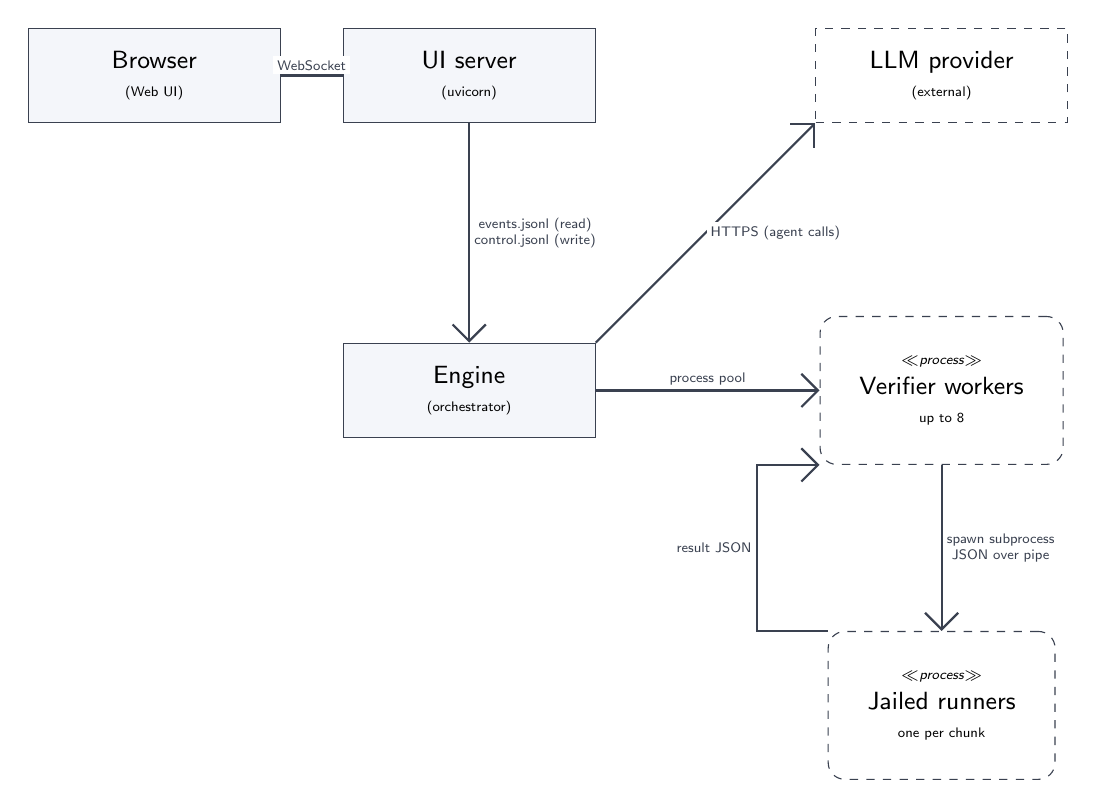
\begin{tikzpicture}[
  node/.style={rectangle, draw=umlline, fill=umlfill, minimum width=3.2cm,
    minimum height=1.2cm, align=center, font=\sffamily\small, inner sep=2.5pt},
  group/.style={rectangle, draw=umlline, fill=white, dashed, rounded corners=6pt,
    inner sep=0.5cm, align=center, font=\sffamily\small},
  ext/.style={node, dashed, fill=white},
  link/.style={-{Straight Barb[length=6pt]}, draw=umlline, line width=0.8pt},
  bidir/.style={draw=umlline, line width=0.8pt},
  lbl/.style={font=\sffamily\tiny, text=umlline, fill=white, inner sep=1.5pt, align=center},
  cap/.style={font=\sffamily\tiny\itshape, text=umlline},
]
  % ------------------------------------------------------------- processes
  \node[node] (browser) at (-6,4)  {Browser\\[-1pt]{\tiny (Web UI)}};
  \node[node] (server)  at (-2,4)  {UI server\\[-1pt]{\tiny (uvicorn)}};
  \node[ext]  (llm)     at (4,4)   {LLM provider\\[-1pt]{\tiny (external)}};
  \node[node] (engine)  at (-2,0)  {Engine\\[-1pt]{\tiny (orchestrator)}};
  \node[group](workers) at (4,0)   {{\tiny\itshape$\ll$process$\gg$}\\Verifier workers\\[-1pt]{\tiny up to 8}};
  \node[group](runners) at (4,-4)  {{\tiny\itshape$\ll$process$\gg$}\\Jailed runners\\[-1pt]{\tiny one per chunk}};

  % ------------------------------------------------------------- paths
  \draw[bidir] (browser.east) -- node[lbl, above] {WebSocket} (server.west);
  \draw[link]  (server.south) -- node[lbl, right] {events.jsonl (read)\\ control.jsonl (write)} (engine.north);
  \draw[link]  (engine.east)  -- node[lbl, above] {process pool} (workers.west);
  \draw[link]  (engine.north east) -- node[lbl, right] {HTTPS (agent calls)} (llm.south west);
  \draw[link]  (workers.south) -- node[lbl, right] {spawn subprocess\\ JSON over pipe} (runners.north);

  % a runner returns its result to the owning worker
  \draw[link]  (runners.north west) -- ++(-0.9,0) |- node[lbl, left, pos=0.25] {result JSON} (workers.south west);
\end{tikzpicture}
\end{document}
